% This file was created by tikzplotlib v0.9.0.
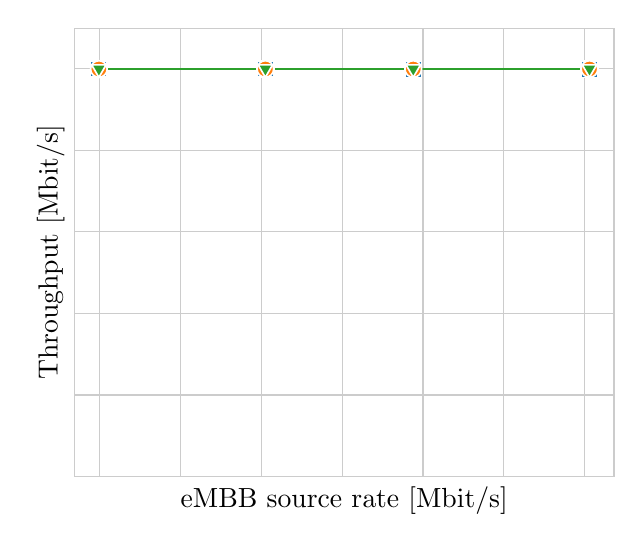
\begin{tikzpicture}

\definecolor{color0}{rgb}{0.12156862745098,0.466666666666667,0.705882352941177}
\definecolor{color1}{rgb}{1,0.498039215686275,0.0549019607843137}
\definecolor{color2}{rgb}{0.172549019607843,0.627450980392157,0.172549019607843}

\begin{axis}[
axis line style={white!80!black},
legend cell align={left},
legend style={fill opacity=0.8, draw opacity=1, text opacity=1, at={(0.03,0.03)}, anchor=south west, draw=white!80!black},
tick align=outside,
x grid style={white!80!black},
xlabel={eMBB source rate [Mbit/s]},
xmajorgrids,
xmajorticks=false,
xmin=96.865, xmax=163.635,
xtick style={color=white!15!black},
y grid style={white!80!black},
ylabel={Throughput [Mbit/s]},
ymajorgrids,
ymajorticks=false,
ymin=0, ymax=1.09971216806957,
ytick style={color=white!15!black},
ytick={0,0.2,0.4,0.6,0.8,1,1.2},
yticklabels={0.0,0.2,0.4,0.6,0.8,1.0,1.2}
]
\path [draw=color0, semithick]
(axis cs:99.9,0.999530852173913)
--(axis cs:99.9,0.999726747826087);

\path [draw=color0, semithick]
(axis cs:120.5,0.999521947826087)
--(axis cs:120.5,0.999717843478261);

\path [draw=color0, semithick]
(axis cs:138.8,0.999504139130435)
--(axis cs:138.8,0.999708939130435);

\path [draw=color0, semithick]
(axis cs:160.6,0.999495234782609)
--(axis cs:160.6,0.999700034782609);

\path [draw=color1, semithick]
(axis cs:99.9,0.999495234782609)
--(axis cs:99.9,0.999717843478261);

\path [draw=color1, semithick]
(axis cs:120.5,0.999512820869565)
--(axis cs:120.5,0.999726747826087);

\path [draw=color1, semithick]
(axis cs:138.8,0.999503916521739)
--(axis cs:138.8,0.999726747826087);

\path [draw=color1, semithick]
(axis cs:160.6,0.999504139130435)
--(axis cs:160.6,0.999726747826087);

\path [draw=color2, semithick]
(axis cs:99.9,0.999504139130435)
--(axis cs:99.9,0.999726747826087);

\path [draw=color2, semithick]
(axis cs:120.5,0.999495234782609)
--(axis cs:120.5,0.999726747826087);

\path [draw=color2, semithick]
(axis cs:138.8,0.999495012173913)
--(axis cs:138.8,0.999717843478261);

\path [draw=color2, semithick]
(axis cs:160.6,0.999512820869565)
--(axis cs:160.6,0.999726747826087);

\addplot [semithick, color0, dash pattern=on 1pt off 1pt, mark=square*, mark size=3, mark options={solid,draw=white}, forget plot]
table {%
99.9 0.9996288
120.5 0.999619895652174
138.8 0.999610991304348
160.6 0.999602086956522
};
\addplot [semithick, color1, mark=*, mark size=3, mark options={solid,draw=white}, forget plot]
table {%
99.9 0.999610991304348
120.5 0.999619895652174
138.8 0.999619895652174
160.6 0.999619895652174
};
\addplot [semithick, color2, dash pattern=on 4pt off 1.5pt, mark=triangle*, mark size=3, mark options={solid,rotate=180,draw=white}, forget plot]
table {%
99.9 0.999619895652174
120.5 0.999619895652174
138.8 0.999610991304348
160.6 0.999619895652174
};
\addplot [semithick, color0, forget plot]
table {%
99.9 0.9996288
120.5 0.999619895652174
138.8 0.999610991304348
160.6 0.999602086956522
};
\addplot [semithick, color1, forget plot]
table {%
99.9 0.999610991304348
120.5 0.999619895652174
138.8 0.999619895652174
160.6 0.999619895652174
};
\addplot [semithick, color2, forget plot]
table {%
99.9 0.999619895652174
120.5 0.999619895652174
138.8 0.999610991304348
160.6 0.999619895652174
};
\end{axis}

\end{tikzpicture}
